\documentclass[aspectratio=169,14pt]{beamer}
\usetheme{default}
\usepackage{fontspec}
\setmainfont{texgyrepagella-regular.otf}[BoldFont=texgyrepagella-bold.otf,ItalicFont=texgyrepagella-italic.otf,BoldItalicFont=texgyrepagella-bolditalic.otf]
\setsansfont{texgyreheros-regular.otf}[BoldFont=texgyreheros-bold.otf,ItalicFont=texgyreheros-italic.otf,BoldItalicFont=texgyreheros-bold.otf,BoldItalicFeatures={FakeSlant=0.2}]
\setmonofont{lmmono10-regular.otf}[Scale=0.85]
\setbeamertemplate{navigation symbols}{}
\usepackage{pgfpages}
\newif\ifpresenter
\ifdefined\PresenterVersion\presentertrue\else\presenterfalse\fi
\ifpresenter
  \setbeameroption{show notes on second screen=right}
  \setbeamertemplate{note page}[plain]
\fi
\usepackage{amsmath,amssymb,bm,booktabs,array,graphicx,xcolor}
\usepackage{tikz,pgfplots,adjustbox,listings,xurl}
\pgfplotsset{compat=1.18}
\usetikzlibrary{arrows.meta,positioning,calc,fit,shapes.geometric,decorations.pathreplacing,patterns}
% UIUC official brand colors, verified 2026-10-23.
% https://brand.illinois.edu/visual-identity/color
\definecolor{IlliniOrange}{HTML}{FF5F05}
\definecolor{IlliniBlue}{HTML}{13294B}
\definecolor{Storm}{HTML}{707372}
\definecolor{LightStorm}{HTML}{C6C7C6}
\definecolor{Industrial}{HTML}{1D58A7}
\definecolor{Patina}{HTML}{007E8E}
\tikzset{>=Stealth, every node/.style={font=\small,text=IlliniBlue}, box/.style={draw=IlliniBlue,rounded corners=2pt,align=center,inner sep=6pt,execute at begin node=\hyphenpenalty10000\relax}, orangebox/.style={box,draw=IlliniOrange,very thick}, edge/.style={->,thick,IlliniBlue}, accent/.style={->,very thick,IlliniOrange}}
\pgfplotsset{every axis/.append style={width=13.5cm,height=6.5cm,axis line style={IlliniBlue},tick label style={font=\small,text=IlliniBlue},label style={font=\small,text=IlliniBlue},legend style={font=\small,draw=none,fill=white},grid style={LightStorm},major grid style={LightStorm},axis lines=left,clip=false}, every axis plot/.append style={thick}}

\definecolor{slidepaper}{RGB}{234,220,201}
\setbeamercolor{background canvas}{bg=slidepaper}
\setbeamercolor{normal text}{fg=IlliniBlue}
\setbeamercolor{frametitle}{fg=IlliniBlue}
\setbeamercolor{title}{fg=IlliniBlue}
\setbeamercolor{item}{fg=IlliniOrange}
\setbeamerfont{frametitle}{size=\large,series=\bfseries}
\setbeamerfont{title}{size=\Large,series=\bfseries}
\setbeamertemplate{itemize item}{\color{IlliniOrange}$\bullet$}
\setbeamertemplate{itemize subitem}{\color{IlliniOrange}\footnotesize$\circ$}
\setbeamercolor{orangerule}{bg=IlliniOrange}
\setbeamertemplate{headline}{\begin{beamercolorbox}[wd=\paperwidth,ht=0.1cm,dp=0.1cm]{orangerule}\end{beamercolorbox}}
\setbeamertemplate{footline}{\begin{beamercolorbox}[wd=\paperwidth,ht=0.1cm,dp=0.1cm]{orangerule}\end{beamercolorbox}}
\setbeamersize{text margin left=0.65cm,text margin right=0.65cm}
\setlength{\leftmargini}{1.1em}
\newenvironment{slidebullets}{\begin{itemize}\setlength\itemsep{0.8em}}{\end{itemize}}
\pgfplotsset{every axis/.append style={legend style={fill=slidepaper}}}
\lstdefinelanguage{CoursePython}{keywords={from,import,for,in,if,else,def,return,assert,True,False,None},sensitive=true,morecomment=[l]{\#},morestring=[b]',morestring=[b]"}
\lstset{language=CoursePython,basicstyle=\ttfamily\small,keywordstyle=\color{IlliniBlue}\bfseries,commentstyle=\color{Storm},stringstyle=\color{IlliniBlue},showstringspaces=false,breaklines=true,columns=fullflexible,keepspaces=true,frame=none,aboveskip=0.7em,belowskip=0.7em}
\newcommand{\E}{\mathbb E}
\newcommand{\Var}{\operatorname{Var}}
\newcommand{\Cov}{\operatorname{Cov}}
\hypersetup{colorlinks=true,urlcolor=IlliniBlue,linkcolor=IlliniBlue}

\title{Marketing Analytics}
\subtitle{Segmentation and Customer Lifetime Value}
\author{By Nathan Yang}
\date{Session 06}
\begin{document}
\begin{frame}
\titlepage
\end{frame}
\begin{frame}{A Retention-Support Decision}
\usebeamercolor[fg]{normal text}
\vfill
\begin{slidebullets}
\item A service team can support only some customers.
\item High baseline value and responsiveness to support are separate quantities.
\item Segments should correspond to feasible service decisions.
\end{slidebullets}
\vfill
\note{A segment with high predicted value may have little incremental response to outreach. The support decision needs the change in future contribution caused by the action, net of its costs.

M4, Section 4.9, Marketing Analytics Lecture Notes. \url{../06_Lecture_Notes/modules/M04_Conjoint_Segmentation_and_CLV.md}}
\end{frame}
\begin{frame}{Customer Features at a Common Date}
\usebeamercolor[fg]{normal text}
\vfill
\begin{slidebullets}
\item Recency is time since the last eligible event.
\item Frequency counts events in a fixed window.
\item Monetary value uses sales or contribution over that window.
\end{slidebullets}
\vfill
\note{Customers with unequal exposure histories can appear different because of observation time. The feature definition must specify eligibility and whether returns affect sales or transaction counts.

M4, Section 4.5, Marketing Analytics Lecture Notes. \url{../06_Lecture_Notes/modules/M04_Conjoint_Segmentation_and_CLV.md}}
\end{frame}
\begin{frame}{K-Means and Similarity}
\usebeamercolor[fg]{normal text}
\noindent Choose $K$ centers for transformed customer features $z_i$.
\medskip
\[
\min_{\mu,c}\sum_i\left\|z_i-\mu_{c(i)}\right\|^2
\]
\medskip
\noindent Scaling the features changes the distance and can change the segments.
\note{K-means minimizes within-cluster squared Euclidean distance. A standardized feature receives a different implicit weight from the raw variable. The transformation is a substantive choice.

M4, Section 4.5, Marketing Analytics Lecture Notes. \url{../06_Lecture_Notes/modules/M04_Conjoint_Segmentation_and_CLV.md}}
\end{frame}
\begin{frame}{Units Change the Nearest Customer}
\usebeamercolor[fg]{normal text}
\centering
\begingroup
\begin{adjustbox}{max width=0.98\textwidth,max totalheight=0.65\textheight}
% Distances within each panel use the stated feature units.
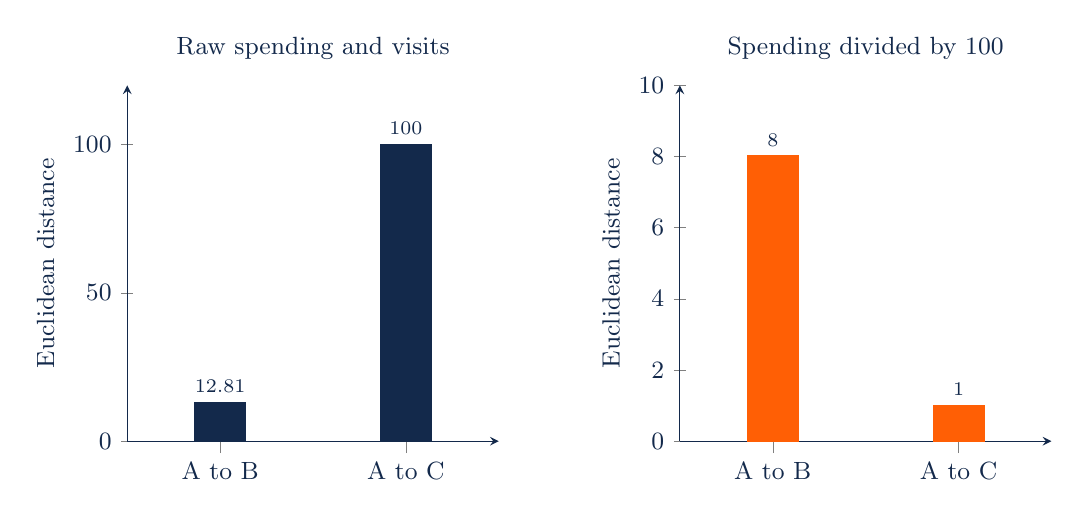
\begin{tikzpicture}
\begin{axis}[name=raw,width=6.3cm,height=6.1cm,xmin=.5,xmax=2.5,ymin=0,ymax=120,ybar,bar width=18pt,xtick={1,2},xticklabels={A to B,A to C},ylabel={Euclidean distance},title={Raw spending and visits},nodes near coords,nodes near coords style={font=\scriptsize}]
\addplot[fill=IlliniBlue,draw=IlliniBlue] coordinates {(1,12.806)(2,100)};
\end{axis}
\begin{axis}[at={(raw.east)},anchor=west,xshift=2.3cm,width=6.3cm,height=6.1cm,xmin=.5,xmax=2.5,ymin=0,ymax=10,ybar,bar width=18pt,xtick={1,2},xticklabels={A to B,A to C},ylabel={Euclidean distance},title={Spending divided by 100},nodes near coords,nodes near coords style={font=\scriptsize}]
\addplot[fill=IlliniOrange,draw=IlliniOrange] coordinates {(1,8.0006)(2,1)};
\end{axis}
\end{tikzpicture}

\end{adjustbox}
\endgroup
\par\medskip
{\small Synthetic customers have unchanged spending and frequency records.\par}
\note{Raw distances compare A=(100,1), B=(110,9), and C=(200,1). The example changes only the spending scale. The preferred business representation depends on the service decision.

M4, Section 4.5, Marketing Analytics Lecture Notes. \url{../06_Lecture_Notes/modules/M04_Conjoint_Segmentation_and_CLV.md}}
\end{frame}
\begin{frame}{Evaluating a Segmentation}
\usebeamercolor[fg]{normal text}
\vfill
\begin{slidebullets}
\item Inspect segment size, profile, and actionable differences.
\item Compare stability across seeds, samples, and periods.
\item Evaluate outcomes that did not mechanically define the clusters.
\end{slidebullets}
\vfill
\note{Within-cluster dispersion declines as K rises. A high-spending cluster will have high spending by construction when spending is an input. Later outcomes provide a more informative descriptive check.

M4, Section 4.6, Marketing Analytics Lecture Notes. \url{../06_Lecture_Notes/modules/M04_Conjoint_Segmentation_and_CLV.md}}
\end{frame}
\begin{frame}{Similarity of Positive Mechanisms}
\usebeamercolor[fg]{normal text}
\noindent For each paper, collect the mechanisms coded as present in a set $A_i$.
\medskip
\[
d_J(i,j)=1-\frac{|A_i\cap A_j|}{|A_i\cup A_j|}
\]
\medskip
\noindent Jaccard distance ignores shared absences. Average linkage compares these distances.
\note{The primary sample is 48 retrieved papers with potential dual use or a reported choice concern. Twelve binary codes include social cues, emotion, disclosure, defaults, and exit friction. A zero code means the mechanism was not coded from reviewed evidence. Missing reviews are excluded. See M4 Section 4.17 for the complete program.

\url{../03_Data_and_Code/Consumer_Agency_Literature/README.md}}
\end{frame}
\begin{frame}{Social Influence is the Largest Cluster}
\usebeamercolor[fg]{normal text}
\centering
\begingroup
\begin{adjustbox}{max width=0.98\textwidth,max totalheight=0.65\textheight}
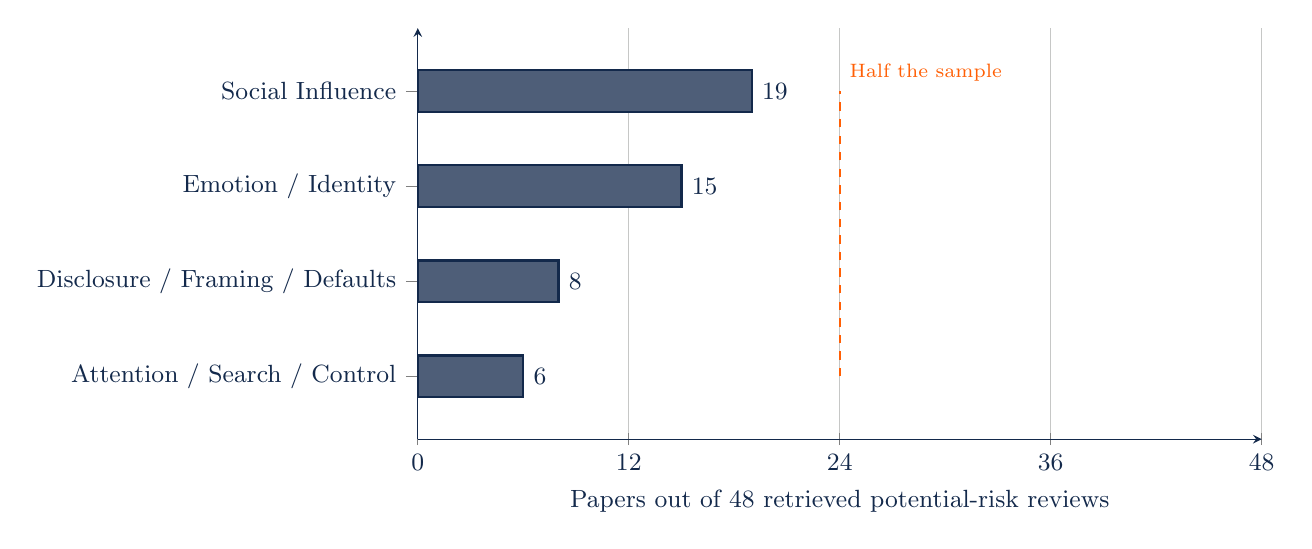
\begin{tikzpicture}
\begin{axis}[
  xbar,width=12.3cm,height=6.8cm,
  xmin=0,xmax=48,xtick={0,12,24,36,48},
  xlabel={Papers out of 48 retrieved potential-risk reviews},
  symbolic y coords={Attention,Disclosure,Emotion,Social},
  ytick=data,
  yticklabels={Attention / Search / Control,Disclosure / Framing / Defaults,Emotion / Identity,Social Influence},
  bar width=15pt,enlarge y limits=.22,
  nodes near coords,nodes near coords align={horizontal},
  nodes near coords style={font=\small,text=IlliniBlue},
  xmajorgrids=true]
\addplot[fill=IlliniBlue!75,draw=IlliniBlue] coordinates {(6,Attention) (8,Disclosure) (15,Emotion) (19,Social)};
\draw[IlliniOrange,dashed,thick] (axis cs:24,Attention)--(axis cs:24,Social);
\node[font=\scriptsize,text=IlliniOrange,anchor=south west] at (axis cs:24,Social) {Half the sample};
\end{axis}
\end{tikzpicture}

\end{adjustbox}
\endgroup
\par\medskip
{\small 48 retrieved potential-risk reviews. Four clusters selected from K=2 through K=8.\par}
\note{The largest cluster contains 39.6\% of the sample. Emotion/identity is the most common overlapping feature at 21 of 48, so feature and cluster rankings differ. Almost all papers in this analysis are coded for inferred dual use. Counts do not measure market prevalence or author intent.

\url{../03_Data_and_Code/Consumer_Agency_Literature/README.md}}
\end{frame}
\begin{frame}[fragile]{Reproduce the Mechanism Grouping}
\usebeamercolor[fg]{normal text}
\noindent Run from the Consumer\_Agency\_Literature folder after installing its requirements.
\begin{lstlisting}
import pandas as pd
from cluster import FEATURES, select_sample, partition
df = pd.read_csv("coded_papers.csv")
sample = select_sample(df, "downloaded_risk")
labels, distances = partition(sample[FEATURES].to_numpy(), 4)
assert len(sample) == 48
\end{lstlisting}
{\small The complete script compares K values, exports profiles, and refits sensitivity samples.\par}
\note{The short snippet reproduces the selected four-cluster partition. The full cluster.py program in M4 Section 4.17 selects K using silhouette scores and checks aggregate counts. Stable paper identifiers preserve traceability to original summaries.

\url{../03_Data_and_Code/Consumer_Agency_Literature/README.md}}
\end{frame}
\begin{frame}{The Coding Changes the Conclusion}
\usebeamercolor[fg]{normal text}
\vfill
\begin{slidebullets}
\item Median subsample agreement: adjusted Rand index 0.794.
\item Changing one feature per paper lowers median agreement to 0.250.
\item The broader abstract-based sample selects eight clusters.
\end{slidebullets}
\vfill
\note{Subsamples contain 80\% of the primary papers and hold K=4 fixed across 200 repetitions. One-bit changes are an imposed sensitivity exercise, retaining a positive feature per paper. These are conditional stability results, not confidence intervals for population harm. The broader 84-paper risk sample is purposefully selected and chooses the upper K boundary.

\url{../03_Data_and_Code/Consumer_Agency_Literature/README.md}}
\end{frame}
\begin{frame}{mHealth Segments Use Earlier Histories}
\usebeamercolor[fg]{normal text}
\centering
\begingroup
\begin{adjustbox}{max width=0.98\textwidth,max totalheight=0.65\textheight}
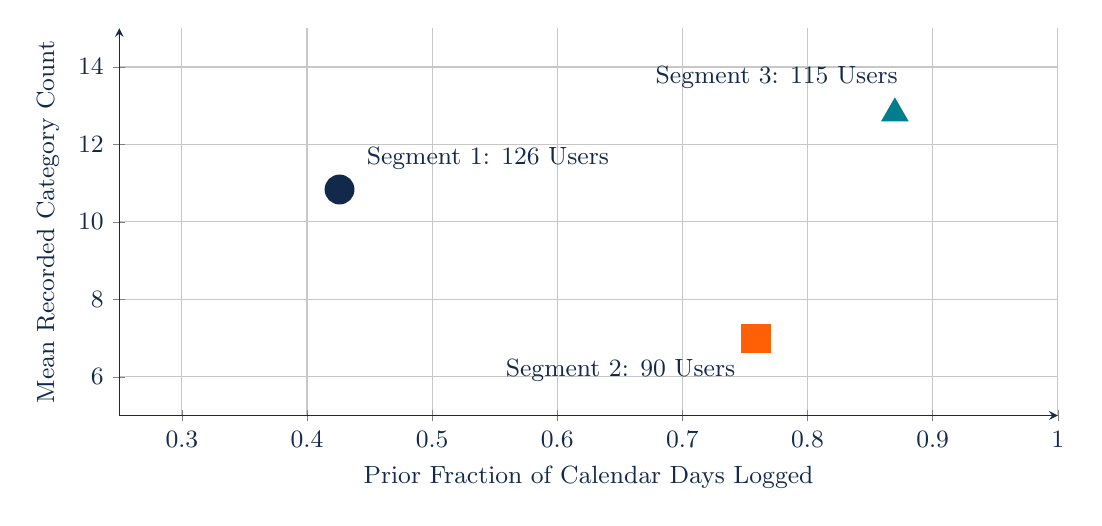
\begin{tikzpicture}
\begin{axis}[xlabel={Prior Fraction of Calendar Days Logged},ylabel={Mean Recorded Category Count},xmin=.25,xmax=1,ymin=5,ymax=15,grid=major]
\addplot[only marks,IlliniBlue,mark=*,mark size=5pt] coordinates {(.425999,10.8354)};
\addplot[only marks,IlliniOrange,mark=square*,mark size=5pt] coordinates {(.758608,6.989)};
\addplot[only marks,Patina,mark=triangle*,mark size=5pt] coordinates {(.869804,12.7997)};
\node[anchor=south west] at (axis cs:.44,11.1) {Segment 1: 126 Users};
\node[anchor=north east] at (axis cs:.75,6.7) {Segment 2: 90 Users};
\node[anchor=south east] at (axis cs:.88,13.2) {Segment 3: 115 Users};
\end{axis}
\end{tikzpicture}

\end{adjustbox}
\endgroup
\par\medskip
{\small Eligible users have at least 30 observed days before July 1.\par}
\note{The representation uses first-half logging fraction, mean category breadth, and mean calorie-share variety. K=3 is imposed for the comparison. The scaler and centers use only the earlier window.

M4, Section 4.11, Marketing Analytics Lecture Notes. \url{../06_Lecture_Notes/modules/M04_Conjoint_Segmentation_and_CLV.md}}
\end{frame}
\begin{frame}{Later Logging by Earlier Segment}
\usebeamercolor[fg]{normal text}
\vfill
\centering
{\small\begin{tabular}{lrrr}
\toprule
Segment & Users & Prior Fraction & Later Fraction \\
\midrule
1 & 126 & 0.426 & 0.338 \\
2 & 90 & 0.759 & 0.594 \\
3 & 115 & 0.870 & 0.654 \\
\bottomrule
\end{tabular}}
\par\medskip
mHealth denominators use 182 earlier and 184 later calendar days.
\vfill
\note{Later absence contributes zero observed days for eligible users. The figures describe persistence in recorded activity. They are not contractual retention rates or effects of a service intervention.

M4, Section 4.11, Marketing Analytics Lecture Notes. \url{../06_Lecture_Notes/modules/M04_Conjoint_Segmentation_and_CLV.md}}
\end{frame}
\begin{frame}{Lifetime Value and Payment Timing}
\usebeamercolor[fg]{normal text}
\noindent Value future contribution conditional on remaining active.
\medskip
\[
\operatorname{CLV}=\sum_{t=1}^{T}\frac{\Pr(\text{active at }t)m_t}{(1+d)^t}-a
\]
\medskip
\noindent The period for margin $m_t$, discounting $d$, and retention must agree.
\note{The acquisition cost a occurs at time zero. This convention excludes immediate contribution. If a current-period contribution is included, it must be added explicitly.

M4, Section 4.7, Marketing Analytics Lecture Notes. \url{../06_Lecture_Notes/modules/M04_Conjoint_Segmentation_and_CLV.md}}
\end{frame}
\begin{frame}{A Stationary Subscription}
\usebeamercolor[fg]{normal text}
\noindent Suppose monthly retention is $r$ and monthly contribution is $m$.
\medskip
\[
\operatorname{CLV}=\frac{mr}{1+d-r}-a
\]
\medskip
\noindent With $m=60$, $d=0.01$, $a=50$, and $r=0.80$, CLV is 178.57 dollars.
\note{The formula assumes constant retention and conditional margin and an infinite horizon, with the first payment one month later. It follows from a convergent geometric series.

M4, Section 4.7, Marketing Analytics Lecture Notes. \url{../06_Lecture_Notes/modules/M04_Conjoint_Segmentation_and_CLV.md}}
\end{frame}
\begin{frame}{Retention Has Nonlinear Value}
\usebeamercolor[fg]{normal text}
\centering
\begingroup
\begin{adjustbox}{max width=0.98\textwidth,max totalheight=0.65\textheight}
% Original synthetic teaching figure; see corresponding module.
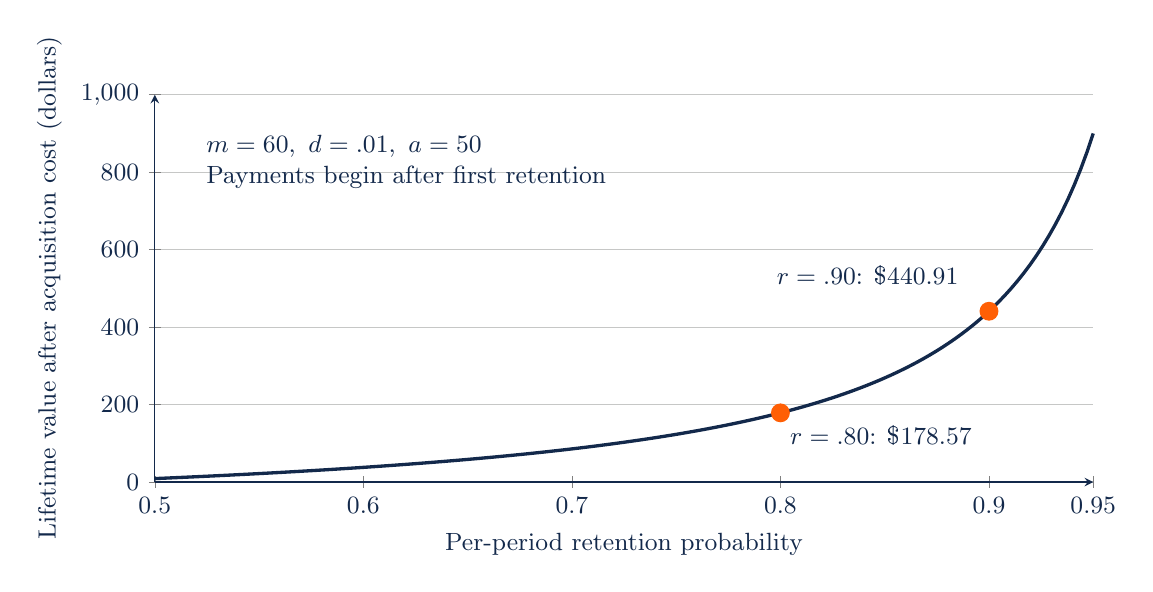
\begin{tikzpicture}
\begin{axis}[xmin=.5,xmax=.95,ymin=0,ymax=1000,xlabel={Per-period retention probability},ylabel={Lifetime value after acquisition cost (dollars)},xtick={.5,.6,.7,.8,.9,.95},ytick={0,200,400,600,800,1000},ymajorgrids=true]
\addplot[IlliniBlue,domain=.5:.95,samples=150,very thick] {60*x/(1.01-x)-50};
\addplot[IlliniOrange,only marks,mark=*,mark size=3pt] coordinates {(.8,178.5714)(.9,440.9091)};
\node[anchor=north west] at (axis cs:.8,170) {$r=.80$: \$178.57};
\node[anchor=south east] at (axis cs:.89,480) {$r=.90$: \$440.91};
\node[align=left,anchor=north west] at (axis cs:.52,920) {$m=60,\ d=.01,\ a=50$\\Payments begin after first retention};
\end{axis}
\end{tikzpicture}

\end{adjustbox}
\endgroup
\par\medskip
{\small Synthetic stationary model. Monthly margin, discounting, and acquisition cost stay fixed.\par}
\note{The high-retention region places more weight on distant contributions. Uncertainty about the persistence of retention and margins can dominate the valuation.

M4, Section 4.7, Marketing Analytics Lecture Notes. \url{../06_Lecture_Notes/modules/M04_Conjoint_Segmentation_and_CLV.md}}
\end{frame}
\begin{frame}[fragile]{A Finite-Sum Check}
\usebeamercolor[fg]{normal text}
\noindent Compare the closed form with 2,000 future monthly payments.
\begin{lstlisting}
m, r, d, a = 60, 0.8, 0.01, 50
closed = m * r / (1 + d - r) - a
finite = sum(m * r**t / (1+d)**t
             for t in range(1, 2001)) - a
assert abs(closed - finite) < 1e-8
\end{lstlisting}
{\small Both calculations give approximately 178.57 dollars.\par}
\note{Matching the two expressions checks the payment convention and arithmetic. It does not establish constant retention as a valid model of a real relationship.

M4, Section 4.7, Marketing Analytics Lecture Notes. \url{../06_Lecture_Notes/modules/M04_Conjoint_Segmentation_and_CLV.md}}
\end{frame}
\begin{frame}{Cancellation and a Logging Gap}
\usebeamercolor[fg]{normal text}
\vfill
\begin{slidebullets}
\item A subscription may record cancellation directly.
\item A 30-day logging gap is an operational activity event.
\item Observation can end before a defined event occurs.
\end{slidebullets}
\vfill
\note{Right censoring preserves the distinction between no observed event by the end of follow-up and an event at the last observation. A logging gap is not proof of permanent departure or paid cancellation.

M4, Section 4.13, Marketing Analytics Lecture Notes. \url{../06_Lecture_Notes/modules/M04_Conjoint_Segmentation_and_CLV.md}}
\end{frame}
\begin{frame}{The Event Definition Changes Survival}
\usebeamercolor[fg]{normal text}
\centering
\begingroup
\begin{adjustbox}{max width=0.98\textwidth,max totalheight=0.65\textheight}
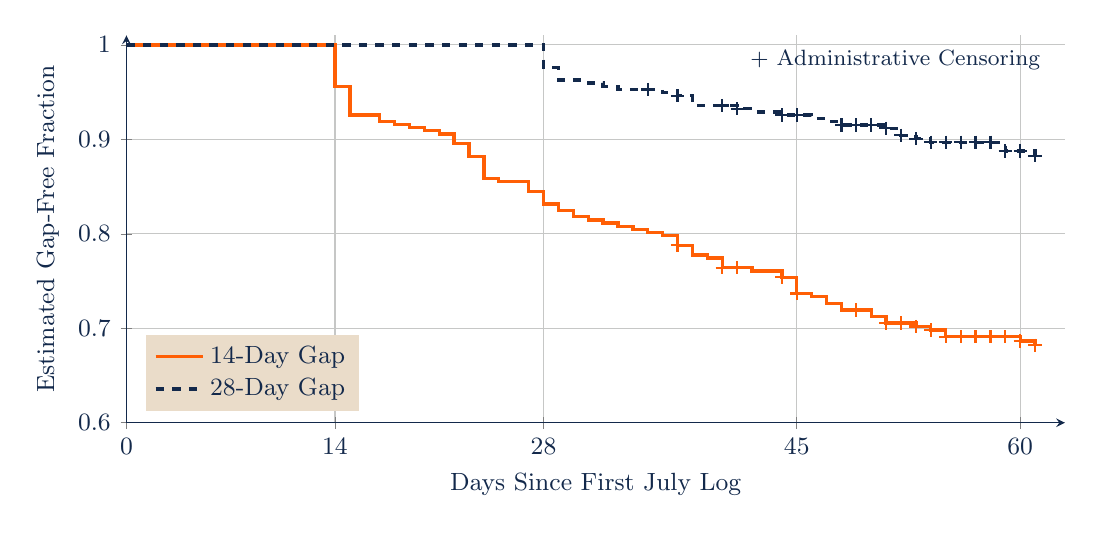
\begin{tikzpicture}
\begin{axis}[xlabel={Days Since First July Log},ylabel={Estimated Gap-Free Fraction},xmin=0,xmax=63,ymin=.6,ymax=1.01,xtick={0,14,28,45,60},ytick={.6,.7,.8,.9,1},yticklabel style={/pgf/number format/fixed,/pgf/number format/precision=1},grid=major,legend style={at={(.02,.03)},anchor=south west}]
\addplot[IlliniOrange,solid,const plot,very thick] coordinates {(0,1) (14,0.95622896) (15,0.92592593) (17,0.91919192) (18,0.91582492) (19,0.91245791) (20,0.90909091) (21,0.90572391) (22,0.89562290) (23,0.88215488) (24,0.85858586) (25,0.85521886) (27,0.84511785) (28,0.83164983) (29,0.82491582) (30,0.81818182) (31,0.81481481) (32,0.81144781) (33,0.80808081) (34,0.80471380) (35,0.80134680) (36,0.79797980) (37,0.78787879) (38,0.77773443) (39,0.77435297) (40,0.76420861) (41,0.76420861) (42,0.76079696) (44,0.75397367) (45,0.73675966) (46,0.73330070) (47,0.72638277) (48,0.71946483) (49,0.71946483) (50,0.71251348) (51,0.70556213) (52,0.70556213) (53,0.70196233) (54,0.69832522) (55,0.69101291) (56,0.69101291) (57,0.69101291) (58,0.69101291) (59,0.69101291) (60,0.68669408) (61,0.68211612)};
\addlegendentry{14-Day Gap}
\addplot[IlliniOrange,only marks,mark=+,mark size=2.4pt,forget plot] coordinates {(37,0.78787879) (40,0.76420861) (41,0.76420861) (44,0.75397367) (45,0.73675966) (49,0.71946483) (51,0.70556213) (52,0.70556213) (53,0.70196233) (54,0.69832522) (55,0.69101291) (56,0.69101291) (57,0.69101291) (58,0.69101291) (59,0.69101291) (60,0.68669408) (61,0.68211612)};
\addplot[IlliniBlue,dashed,const plot,very thick] coordinates {(0,1) (28,0.97643098) (29,0.96296296) (31,0.95959596) (32,0.95622896) (33,0.95286195) (35,0.95286195) (36,0.94948301) (37,0.94610407) (38,0.93593090) (40,0.93593090) (41,0.93252752) (42,0.92911167) (44,0.92569582) (45,0.92569582) (46,0.92222879) (47,0.91876177) (48,0.91529474) (49,0.91529474) (50,0.91529474) (51,0.91176078) (52,0.90440787) (53,0.90065514) (54,0.89687088) (55,0.89687088) (56,0.89687088) (57,0.89687088) (58,0.89687088) (59,0.88771913) (60,0.88771913) (61,0.88264645)};
\addlegendentry{28-Day Gap}
\addplot[IlliniBlue,only marks,mark=+,mark size=2.4pt,forget plot] coordinates {(35,0.95286195) (37,0.94610407) (40,0.93593090) (41,0.93252752) (44,0.92569582) (45,0.92569582) (48,0.91529474) (49,0.91529474) (50,0.91529474) (51,0.91176078) (52,0.90440787) (53,0.90065514) (54,0.89687088) (55,0.89687088) (56,0.89687088) (57,0.89687088) (58,0.89687088) (59,0.88771913) (60,0.88771913) (61,0.88264645)};
\node[anchor=north east,font=\footnotesize] at (axis cs:62,1.005) {+ Administrative Censoring};
\end{axis}\end{tikzpicture}

\end{adjustbox}
\endgroup
\par\medskip
{\small mHealth time-to-gap analysis uses a stated gap definition and observation horizon.\par}
\note{Changing the gap length changes the event being measured. Survival of recorded activity should remain separate from contractual renewal in financial calculations.

M4, Section 4.13, Marketing Analytics Lecture Notes. \url{../06_Lecture_Notes/modules/M04_Conjoint_Segmentation_and_CLV.md}}
\end{frame}
\begin{frame}{Endpoint and Continuous Retention}
\usebeamercolor[fg]{normal text}
\vfill
\begin{slidebullets}
\item Endpoint retention allows customers to leave and return.
\item Continuous retention requires uninterrupted presence.
\item Acquisition can include first entry, return, or switching.
\end{slidebullets}
\vfill
\note{A starting-provider cohort is fixed at the initial period. The same-provider, other-provider-only, and no-paid-provider states distinguish platform retention from category participation. Multiple providers require explicit overlap handling.

M4, Section 4.14, Marketing Analytics Lecture Notes. \url{../06_Lecture_Notes/modules/M04_Conjoint_Segmentation_and_CLV.md}}
\end{frame}
\begin{frame}{Coding Exercise: Segments and Value}
\usebeamercolor[fg]{normal text}
\vfill
\begin{slidebullets}
\item Fit feature scaling and segments on an earlier period.
\item Describe a later period without refitting the groups.
\item Vary assumed paid retention in a separate CLV calculation.
\end{slidebullets}
\vfill
\note{The small CLV calculation is ../03\_Data\_and\_Code/Lecture\_Examples/session\_examples.py S06. The real mHealth m04.py example and GenAI cohort program keep behavioral measurements separate from imposed financial inputs.

M4, Section 4.11, Marketing Analytics Lecture Notes. \url{../06_Lecture_Notes/modules/M04_Conjoint_Segmentation_and_CLV.md}}
\end{frame}
\begin{frame}{Retention and Effective Cancellation}
\usebeamercolor[fg]{normal text}
\vfill
\begin{slidebullets}
\item High paid retention can reflect satisfaction or difficulty leaving.
\item Measure cancellation completion and unwanted subsequent charges.
\item Evaluate customer value alongside the seller's lifetime-value objective.
\end{slidebullets}
\vfill
\note{A customer who prefers cancellation can remain subscribed because of friction. The consumer-value comparison requires independent evidence about that preference and the available procedure.

M8, Section 8.14, Marketing Analytics Lecture Notes. \url{../06_Lecture_Notes/modules/M08_Current_Topics_and_Integrated_Decisions.md}}
\end{frame}
\begin{frame}{Retention Discussion}
\usebeamercolor[fg]{normal text}
\vfill
\begin{slidebullets}
\item What action differs across the proposed segments?
\item Does a customer's absence represent churn or censoring?
\item Which retention assumption changes the support decision?
\end{slidebullets}
\vfill
\note{A useful recommendation identifies the response to intervention as well as baseline value. Cluster membership alone does not establish the effectiveness of differentiated support.

M4, Section 4.9, Marketing Analytics Lecture Notes. \url{../06_Lecture_Notes/modules/M04_Conjoint_Segmentation_and_CLV.md}}
\end{frame}
\end{document}
